%Para hacer informe con portada utilizamos report

\documentclass[12pt]{report}

\usepackage[a4paper]{geometry}
\usepackage[myheadings]{fullpage}
\usepackage{fancyhdr}
\usepackage{lastpage}
\usepackage{graphicx, wrapfig, subcaption, setspace, booktabs}
\usepackage[T1]{fontenc}
\usepackage[font=small, labelfont=bf]{caption}
\usepackage{fourier}
\usepackage[protrusion=true, expansion=true]{microtype}
\renewcommand\thesection{\arabic{section}}

%Paquete para hipervinculos
\usepackage[colorlinks=true]{hyperref}
\hypersetup{
    colorlinks=true,
    linkcolor=black,
    filecolor=magenta,      
    urlcolor=blue,
}

%Para qué los subtítulos aparezcan en español
\usepackage[spanish]{babel}
\usepackage[utf8]{inputenc}
\usepackage{sectsty}
\usepackage{url, lipsum}
\usepackage{tabularx}
\usepackage{float}

%--------------------------------------------------
%Para agregar citas en apa
%Para citar se usa el comando \cite{}
%Las referencias se modifican en el archivo sample.bib
\usepackage{apacite}
%----------------------------------------------

\newcommand{\HRule}[1]{\rule{\linewidth}{#1}}
\onehalfspacing
\setcounter{tocdepth}{5}
\setcounter{secnumdepth}{5}

%-------------------------------------------------------------------------------
%Encabezado y pie de pagina y numeracion
%\fancyhead para encabezado
%\fancyfoot para pie de pagina
% L para izquierda, left
% R para derecha, right
% C para centro, center
%-------------------------------------------------------------------------------
\pagestyle{fancy}
\fancyhf{}
\setlength\headheight{15pt}
%\fancyhead[L]{\chaptername \ \thechapter} 
\fancyhead[L]{Universidad de las Fuerzas Armadas ESPE}
\fancyfoot[R]{\thepage}

\begin{document}


%-------------------------------------------------------------------------------
% Portada
%-------------------------------------------------------------------------------
\title{ \normalsize Universidad de las Fuerzas Armadas ESPE \\
		Technologies de software para electrónica\\
		Producto de Unidad
		\\ [2.0cm]
		\HRule{0.5pt} \\
		\LARGE \textbf{Comunicacion Serial} %para que quede encerrado en las lineas
		\HRule{2pt} \\ [0.5cm]
		\normalsize \today \vspace*{5\baselineskip}}

\date{}

\author{
		 Socasi Bryan, Viera Katherine, Yanez Danilo \\ 
		 basocasi@espe.edu.ec\\
		 kaviera1@espe.edu.ec\\
		 djyanez1@espe.edu.ec
		 }
%se debe incluir el comando \maketitle para hacer 
\maketitle

%Para hacer el indice solo es necesario agregar 
\tableofcontents
\newpage

%-------------------------------------------------------------------------------
% Section title formatting
%\sectionfont{\scshape}
%-------------------------------------------------------------------------------

%-------------------------------------------------------------------------------
% BODY
%-------------------------------------------------------------------------------
\section{Introducción}
La evolución de la tecnología en las últimas décadas ha permitido generar nuevos protocolos y dispositivos para la transmisión de datos entre una computadora y un periférico, en sus inicios alrededor de los años 60 esta transmisión de información se daba a través de puertos seriales enviando datos bit a bit con tiempo de espera prolongado, después en 1998 fue reemplazada por puertos USB’s que tenían mejores características y mayor eficiencia. 
Actualmente los individuos no tienen pleno conocimiento sobre los fundamentos o la estructura base que permitió que la comunicación pueda darse como se la conoce ahora, sin embargo, es muy importante entender los inicios en esta área especialmente para los estudiantes de ingeniería en electrónica, pues de esta manera se logrará entender la diversidad que ha existido a lo largo del tiempo y cómo funciona cada “cosa” que utilizamos. 
Relacionando los temas aprendidos en clase se desarrolla un trabajo de investigación que involucra la comunicación serial entre dos PC a través de una interfaz gráfica desarrollada con lenguaje de programación Java, controlada por un arduino.
\newpage

\section{Objetivos}
\subsection{Objetivo general}
Desarrollar una aplicación en comunicación serial mediante el uso de Arduino y Java para poder controlar sensores y actuadores, a través de dos computadoras, utilizando programación en Java.

\subsection{Objetivos específicos}
\begin{itemize}
\item Conocer el debido funcionamiento de la comunicación de puertos seriales. 
\item Diseñar un programa que permita crear un programa de manera eficaz y visual.
\item Realizar pruebas, del funcionamiento de la aplicación mediante la conexión de la Comunicación Serial de los sensores y actuadores.
\end{itemize}

\section{Estado del arte}
\subsection{Java}
En (Cisco systems, 2016) se indica qué es Java y su programación orientada a objetos, elementos del lenguaje Java, operadores y estructuras de control del lenguaje Java, fundamentos de definición y uso de clases, sistema, cadenas, cadena de buffer, math y otras clases de envoltura, arrays, clases y herencia, cómo comprender y usar los paquetes, creación de interfaces gráficas de usuario con AWT, applets y gráficos, excepciones, archivos, flujos, entrada y salida, colecciones, hilos.\\
En (Wielenga, 2015) se indicó como fue el comienzo de la plataforma Neatbeans IDE para programar códigos Java,  de esta manera se sabe que es un entorno de desarrollo gratuito y de código abierto que permite el uso de un amplio rango de tecnologías de desarrollo tanto para escritorio, como aplicaciones Web, o para dispositivos móviles. Da soporte a las siguientes tecnologías, entre otras: Java, PHP, Groovy, C/C++, HTML5. Además, puede instalarse en varios sistemas operativos: Windows, Linux, Mac OS
.\\

\subsection{Arduino}
En (Albatish, Mosa, & Abu , 2018) se encontró información sobre cómo enfrentar alguna dificultad al tratar con la plataforma Arduino mediante la descripción del diseño de un sistema de tutoría inteligente basado en escritorio. La idea principal de este sistema es una introducción sistemática al concepto de plataforma Arduino. El sistema muestra las placas de circuito de Arduino y un entorno de desarrollo de fuente abierta y una biblioteca para escribir código para controlar el tema de la placa de la plataforma Arduino.
Lo que nos indica en (Pan & Zhu, 2018) es que un sensor es "un dispositivo que detecta una variación en la energía de entrada para producir una variación en otra o la misma forma de energía". Por tanto, implementarlos con arduino, es una manera muy interesante de realizar este tipo de proyectos, de esta manera, en este artículo se describe aspectos importantes de su uso.\\

\subsection{Comunicación Serial}
En el artículo de (Padrón, Prieto, Herrera, & Velazquez, 2018) se indica una aplicación importante con la comunicación serial pues debido a la naturaleza inherente a las comunicaciones móviles, diversos factores influyen en la calidad de los servicios que se desarrollan para los dispositivos de enlace cuando son fabricados, en los cuales no se encuentran técnicas y procedimientos de seguridad implementados en comparación con dispositivos fijos o de escritorio actuales. En este trabajo se presenta la implementación del algoritmo criptográfico por bloques "Advanced Encryption Standard" (AES) de 128 bits, para una comunicación serial entre dos tarjetas Spartan 3E fabricadas por Xilinx. Este algoritmo público según la FIPS-197 es el estándar para muchas aplicaciones en Seguridad Informática tanto en Software como Hardware. Este método criptográfico sigue siendo un mecanismo para implementar los servicios de seguridad recomendados en la ISO 7498-2.


\section{Marco teórico}
\subsection{Arduino Uno}
Arduino UNO es una placa electrónica basada en el microcontrolador ATmega 328. Cuenta con 14 pines digitales que pueden ser entradas o salidas de los cuales 6 pueden ser usados como salidas PWM, 6 entradas analógicas, un cristal oscilador de 16 MHz, una conexión USB, un conector de alimentación, una cabecera ICSP y un botón de reinicio. La placa electrónica tiene todo lo necesario para proporcionar soporte al microcontrolador, basta con conectar la placa a una computadora con un cable USB o a un adaptador AC-DC o a una batería para empezar.

\begin{center}
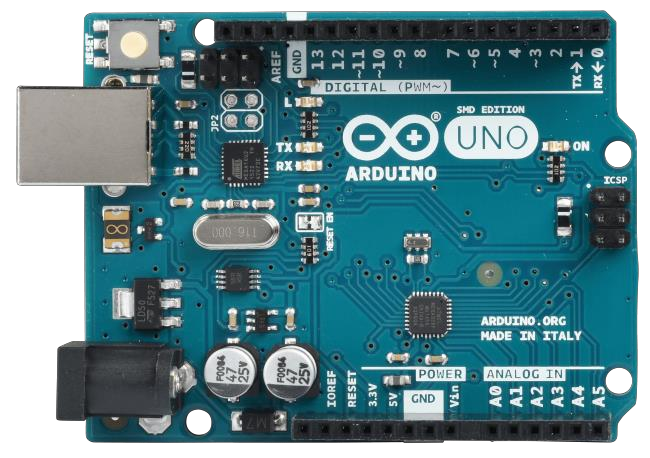
\includegraphics[scale=0.3]{Documento/Figuras/fig1.png}
\begin{scriptsize}\\ 
Fig 1. Arduino Uno
\end{scriptsize}
\end{center}

La tarjeta Arduino UNO SMD difiere de todas las placas anteriores ya que no utiliza el chip FTDI USB serie. Por el contrario, cuenta con el ATmega16U2 programado como un conversor de USB a serie.  “Uno” significa uno en italiano y se llama así por motivos de la próxima versión de Arduino 1.0. La tarjeta Uno y la versión 1.0 serán la versión de referencia de Arduino para seguir adelante. La tarjeta Uno es la última en una serie de placas USB de Arduino, y el modelo de referencia para la plataforma Arduino. (Crespo, 2016)

\subsection{Definición de pines}
\begin{center}
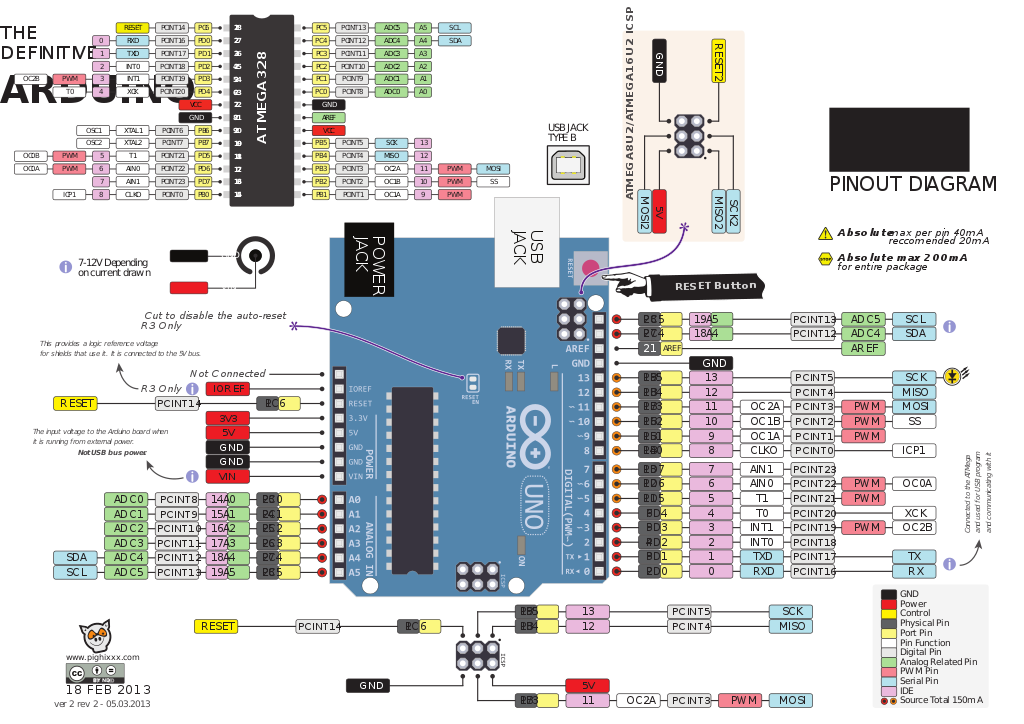
\includegraphics[scale=0.38]{Documento/Figuras/fig2.png}
\begin{scriptsize}\\ 
Fig 1. Definición de pines Arduino Uno
\end{scriptsize}
\end{center}

\subsubsection{Especificaciones Técnicas}
\begin{table}[h]
\caption{Especificaciones de la tarjeta Arduino UNO SMD parte 1}
\begin{center}
\begin{tabular}{|c|c|}
\hline
Microcontrolador & ATmega328\\ \hline
Voltaje de Operación & 5V\\ \hline
Voltaje de alimentación (recomendado) & 7-12V \\ \hline
Voltaje de alimentación (limite) & 6-20V \\ \hline
Pines Digitales E/S	& 14(6 proveen salida PWM) \\ \hline
Pines entradas análogas	& 6 \\ \hline
Corriente DC por pin E/S &  40mA\\ \hline
Voltaje de Corriente DC por el pin de 3.3V & 50mA \\ \hline
\end{tabular}
\end{center}
\end{table}

\begin{table}[h]
\caption{Especificaciones de la tarjeta Arduino UNO SMD parte 2}
\begin{center}
\begin{tabular}{|c|c|}
\hline
Memoria Flash & 32KB de los cuales 0.5KB son usados por el gestor de arranque
\\ \hline
SRAM & 2KB (ATmeta328P)\\ \hline
EEPROM & 16MHz \\ \hline
Reloj & 16MHz \\ \hline
LED BUILTIN	& 13 \\ \hline
Longitud	& 53.4 mm \\ \hline
Ancho & 53.4 mm \\ \hline
Peso & 25 g \\ \hline
\end{tabular}
\end{center}
\end{table}
 
\subsection{Java}
Es un lenguaje de programación de propósito general, concurrente, orientado a objetos que fue diseñado específicamente para tener tan pocas dependencias de implementación como fuera posible. Su intención es permitir que los desarrolladores de aplicaciones escriban el programa una vez y lo ejecuten en cualquier dispositivo, lo que quiere decir que el código que es ejecutado en una plataforma no tiene que ser recompilado para correr en otra. Java es, a partir de 2012, uno de los lenguajes de programación más populares en uso, particularmente para aplicaciones de cliente-servidor de web.
El lenguaje de programación Java fue originalmente desarrollado por James Gosling de Sun Microsystems publicado en 1995 como un componente fundamental de la plataforma Java de Sun Microsystems. Su sintaxis deriva en gran medida de C y C++, pero tiene menos utilidades de bajo nivel que cualquiera de ellos. Las aplicaciones de Java son generalmente compiladas a bytecode (clase Java) que puede ejecutarse en cualquier máquina virtual Java (JVM) sin importar la arquitectura de la computadora subyacente.
La compañía Sun desarrolló la implementación de referencia original para los compiladores de Java, máquinas virtuales, y librerías de clases en 1991 y las publicó por primera vez en 1995. A partir de mayo de 2007, en cumplimiento con las especificaciones del Proceso de la Comunidad Java, Sun volvió a licenciar la mayoría de sus tecnologías de Java bajo la Licencia Pública General de GNU. Otros también han desarrollado implementaciones alternas a estas tecnologías de Sun, tales como el Compilador de Java de GNU y el GNU Classpath. (Itcea, 2017)

\begin{center}

\includegraphics[scale=0.2]{Documento/Figuras/fig3.png}
\begin{scriptsize}\\ 
Fig 2. Lenguaje de Programacion JAVA
\end{scriptsize}
\end{center}

\subsection{API Java Comunication}
La API de Java Communications es una extensión de Java que facilita el desarrollo de aplicaciones de comunicaciones independientes de plataforma para tecnologías como Smart Cards, sistemas integrados y dispositivos de punto de venta, dispositivos de servicios financieros, fax, módems, terminales de pantalla y equipos robóticos.
La API de comunicaciones de Java también conocida como javax.comm permite a las aplicaciones el acceso al hardware RS-232 (puertos serie) y un acceso limitado a IEEE-1284 (puertos paralelos), modo SPP. (Itcea, 2017)

\subsection{Características serial API}
 \begin{itemize}
     \item Enumeración de puertos (mapeo de puertos configurables por el administrador y el usuario)
     \item Configuración del puerto (velocidad en baudios, velocidad, bits de parada, paridad)
     \item Acceso a señales estándar DTR, CD, CTS, RTS y DSR EIA232
     \item Transferencia de datos a través de puertos RS-232
     \item Opciones de control de flujo de hardware y software.
     \item 	Control de umbral de buffer de recepción.
     \item Opción de evento asincrónico para la notificación de:
     \begin{itemize}
         \item Datos disponibles en un puerto RS232.
         \item Cambios de nivel de línea de hardware de puerto.
         \item Cambios en la propiedad de puerto de una solo JVM.
     \end{itemize}
 \end{itemize}
 
\subsection{Sensores}
Es un concepto genérico que hace referencia a diferentes tipos de sensores, esto se entiende tanto las unidades que emite una señal analógica, como las unidades que emite una señal binaria (encendido o apagado).

\begin{center}
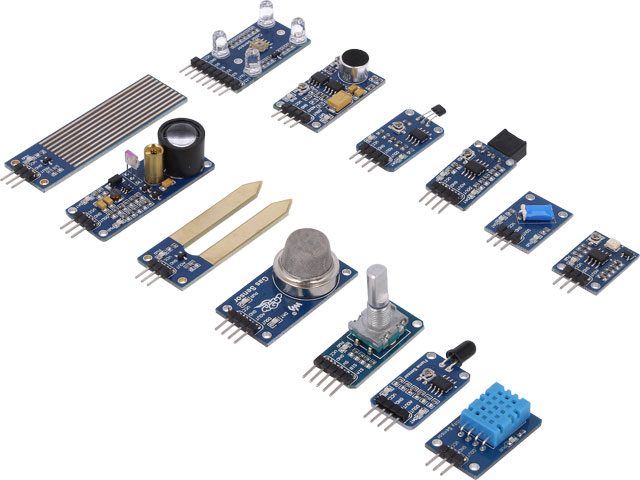
\includegraphics[scale=0.33]{Documento/Figuras/fig4.jpg}
\begin{scriptsize}\\ 
Fig 3. Sensores Electrónicos.
\end{scriptsize}
\end{center}

Convierte una magnitud física en una magnitud eléctrica, existe una gama de diferentes productos de sensores para diferentes magnitudes físicas.

\subsubsection{Sensor de temperatura}
El DHT11 es un sensor de temperatura y humedad el cual dispone de una salida digital calibrada. Su tecnología garantiza la alta fiabilidad y una excelente estabilidad a largo plazo. Es compatible con la tecnología Arduino, PIC, AVR, COP, DSP, STM32, etc.

 \begin{center}
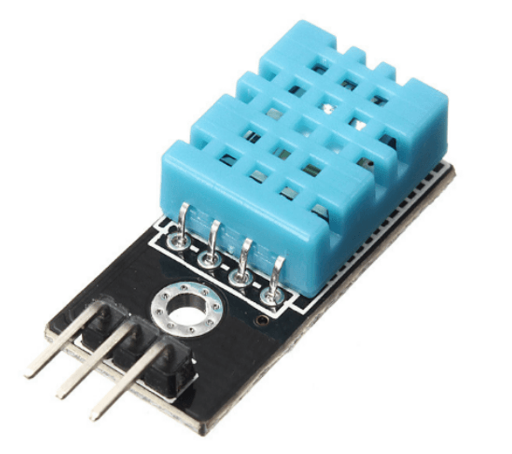
\includegraphics[scale=0.38]{Documento/Figuras/fig5.png}
\begin{scriptsize}\\ 
Fig 4. Sensor de Temperatura
\end{scriptsize}
\end{center}

Características:
\begin{itemize}
    \item Compatible con sistemas
    electrónicos operando entre 3v-5v 
    \item Corriente máxima de 2.5 mA cuando se realiza la conversión.
    \item Humedad relativa: 0-80% (±5%)
    \item Temperatura: 0-50°C (±2°C)
    \item Tiempo de respuesta: ≈10 segundos
    \item 4 pines de conexión 
    \item No requiere componentes activos externos.
\end{itemize}

\subsubsection{Sensor de proximidad}
Puede detectar objetos metálicos que se acercan al sensor, sin tener contacto físico con los mismos. Los sensores de proximidad inductivos se clasifican más o menos en los siguientes tres tipos, de acuerdo con su principio de funcionamiento: el tipo de oscilación de alta frecuencia que utiliza la inducción electromagnética; el tipo magnético que emplea un imán; y el tipo de capacitancia que aprovecha los cambios en la capacidad eléctrica.

 \begin{center}
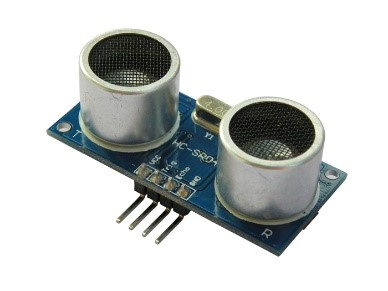
\includegraphics[scale=1.1]{Documento/Figuras/fig6.jpg}
\begin{scriptsize}\\ 
Fig 5. Sensor de Proximidad
\end{scriptsize}
\end{center}

Utiliza este sensor ultrasónico en tus proyectos con Arduino o microcontroladores, con el podrás medir la proximidad de algún objeto.

Características:
\begin{itemize}
    \item Detección de la gama: 3 cm - 4 m
    \item Mejor en ángulo de 30 grados
    \item Fuente de alimentación de 5 Vdc
    \item Transductor Dual
\end{itemize}

\subsubsection{Sensor de CO2}
Es un sensor de gas semiconductor sintonizado para detectar monóxido de carbono. Se encuentra en la misma familia de dispositivos que el sensor detector de humo, que mide el cambio en la conductividad de la superficie del dióxido de estaño en presencia de monóxido de carbono. Este sensor tiene una alta sensibilidad y un rápido tiempo de respuesta. La salida del sensor es una resistencia analógica.

\begin{center}
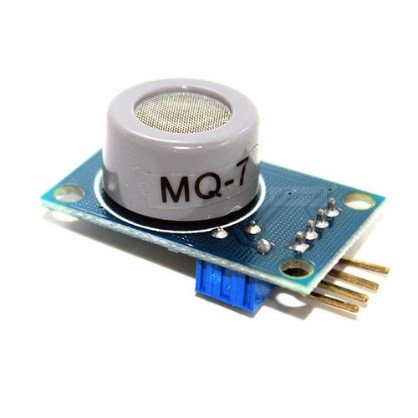
\includegraphics[scale=0.98]{Documento/Figuras/fig7.jpg}
\begin{scriptsize}\\ 
Fig 6. Sensor de CO2.
\end{scriptsize}
\end{center}

\begin{table}[h]
\caption{Caracteristicas}
\begin{center}
\begin{tabular}{|c|c|}
\hline
Zona de detección & 10 a 1000ppmm
\\ \hline
Voltaje de operación & 5V DC \\ \hline
Resistencia de carga & regulable \\ \hline
Sensibilidad &  Mayor al 3\% \\ \hline
Tiempo de respuesta	& Menos 1s \\ \hline
Resistencia al calentamiento & 33 Ohm \\ \hline
Tiempo de calentamiento & 60s (alto) 90s (bajo) \\ \hline
Condiciones: Temperatura ambiente	& -20C a + 50C \\ \hline
Humedad & 95\% RH \\ \hline
Contenido de oxígeno & 21\% \\ \hline
\end{tabular}
\end{center}
\end{table}



 \section{Diagramas}
\subsection{Diagrama de bloques}

 \begin{center}
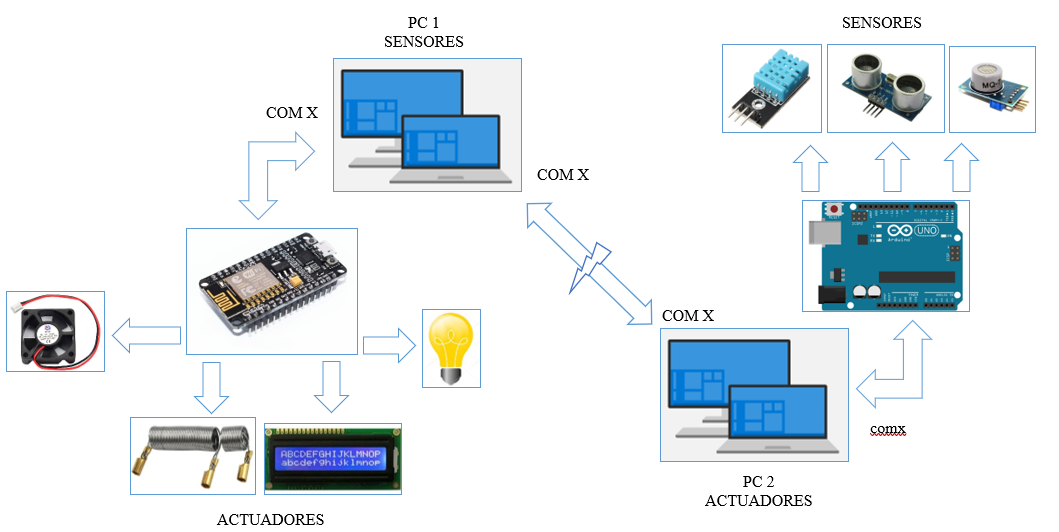
\includegraphics[scale=0.58]{Documento/Figuras/fig8.PNG}
\begin{scriptsize}\\ 
Fig 8. Diagrama de bloques de la Comunicación Serial
\end{scriptsize}
\end{center}

\subsection{Diagrama UML Sensores}
 \begin{center}
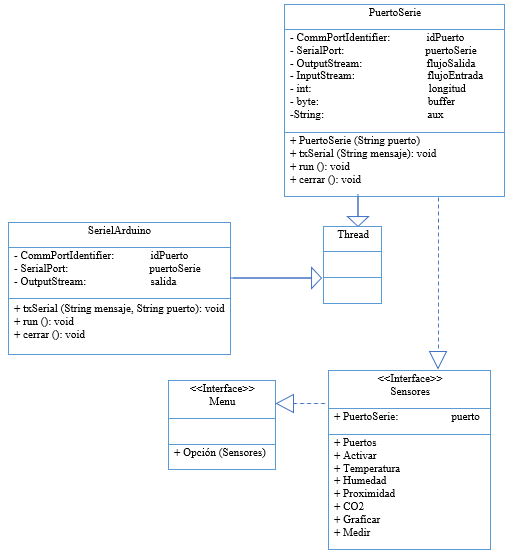
\includegraphics[scale=0.58]{Documento/Figuras/fig9.PNG}
\begin{scriptsize}\\ 
Fig 9. Diagrama UML para los Sensores
\end{scriptsize}
\end{center}

\subsection{Diagrama UML Actuadores}
 \begin{center}
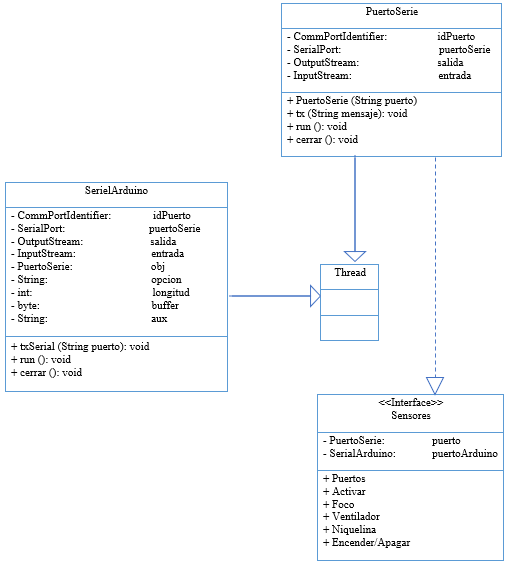
\includegraphics[scale=0.58]{Documento/Figuras/fig10.PNG}
\begin{scriptsize}\\ 
Fig 10. Diagrama UML para los Actuadores
\end{scriptsize}
\end{center}


 \section{Lista de componentes}
\begin{table}[h]
\caption{Lista de componentes}
\begin{center}
\begin{tabular}{|c|c|}
\hline
Fotografía & Nombre\\
\hline
 \begin{center}
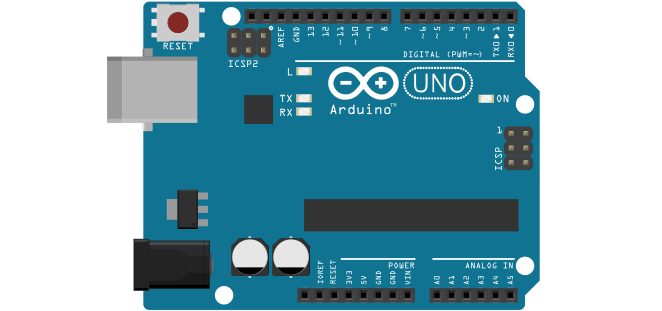
\includegraphics[scale=0.15]{Documento/Figuras/Arduino.png}
\begin{scriptsize}\\ 

\end{scriptsize}
\end{center} & Tarjeta de  desarrollo Arduino\\
\hline
 \begin{center}
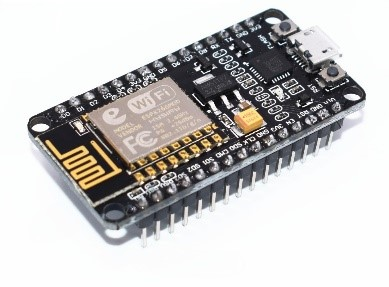
\includegraphics[scale=0.35]{Documento/Figuras/ESP8266.jpg}
\begin{scriptsize}\\ 

\end{scriptsize}
\end{center} & Tarjeta de desarrollo ESP8266\\
\hline
 \begin{center}
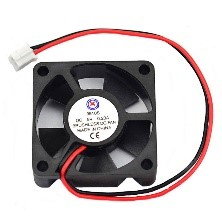
\includegraphics[scale=0.35]{Documento/Figuras/Ventilador.jpg}
\begin{scriptsize}\\ 

\end{scriptsize}
\end{center} & Ventilador  \\
\hline
 \begin{center}
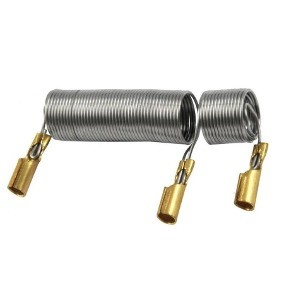
\includegraphics[scale=0.35]{Documento/Figuras/Niquelina.jpg}
\begin{scriptsize}\\ 

\end{scriptsize}
\end{center} & Niquelina\\
\hline
 \begin{center}
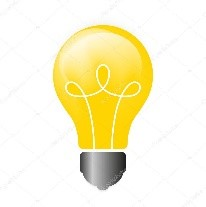
\includegraphics[scale=0.35]{Documento/Figuras/Foco.jpg}
\begin{scriptsize}\\ 

\end{scriptsize}
\end{center} & Foco \\
\hline
 \begin{center}
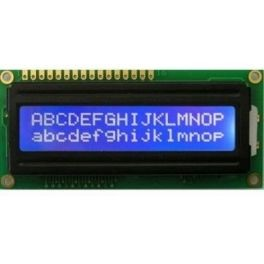
\includegraphics[scale=0.35]{Documento/Figuras/LCD.jpg}
\begin{scriptsize}\\ 

\end{scriptsize}
\end{center} & LCD \\
\hline
 \begin{center}
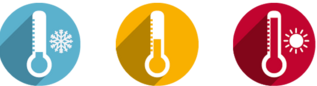
\includegraphics[scale=0.35]{Documento/Figuras/Temperatura.png}
\begin{scriptsize}\\ 

\end{scriptsize}
\end{center} & Sensor de temperatura DHT11 \\
\hline
 \begin{center}
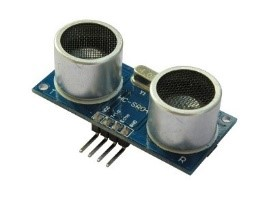
\includegraphics[scale=0.35]{Documento/Figuras/Proximidad.jpg}
\begin{scriptsize}\\ 

\end{scriptsize}
\end{center} & Sensor de proximidad \\
\hline
 \begin{center}
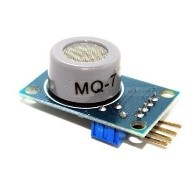
\includegraphics[scale=0.35]{Documento/Figuras/CO2.jpg}
\begin{scriptsize}\\ 

\end{scriptsize}
\end{center} & Sensor de CO2 MQ7\\
\hline
\end{tabular}
\end{center}
\end{table}

 \section{EXPLICACIÓN DEL CÓDIGO FUENTE}
\subsection{Comunicación Serial}
Usaremos el API Java Communications (COMM) que nos permitirá manejar el puerto serie, y así comunicarnos con el otro computador. 
También usaremos cables adaptadores USB a DB9 y el más importante, un cable DB9 cruzado para que el envió de bits se realice correctamente.
Para usar el api de comunicaciones de java necesitaremos de una librería que contiene las clases para manejar los puertos, estos archivos se deben incluir en la carpeta donde se encuentra el Java instalado, siguiendo las siguientes direcciones:
\begin{itemize}
    \item Comm.jar \textbackslash jdk\textbackslash jre\textbackslash lib\textbackslash ext
    \item Win32com.dll  \textbackslash jdk\textbackslash bin y en \textbackslash Windows\textbackslash system32
    \item Javax.comm.properties \textbackslash jdk\textbackslash jre\textbackslash lib
\end{itemize}
	
Para el código necesitaremos importar la librería mencionada anteriormente
\\
\begin{center}
    import javax.comm.*; 
\end{center}
\\
A continuación tenemos que declarar las clases necesarias para manejar los puertos con sus respectivas variables asignadas, hay que tener en cuenta que la comunicación que usaremos es FULL-DUPLEX, ya que enviaremos y recibiremos información entre ambos computadores.
\begin{center}
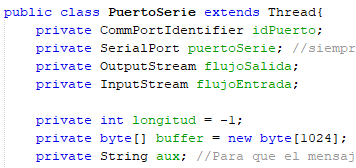
\includegraphics[scale=0.8]{Documento/Figuras/1.PNG}
\begin{scriptsize}
\\ 
\end{scriptsize}
\end{center}
En donde la Clase CommPortIdentifier administrara la comunicación con los puertos, el acceso a estos y determina y están disponibles o ocupados para establecer la comunicación.
La clase SerialPort hereda de la clase abstracta CommPort por lo tanto cuenta con sus métodos pero además posee métodos específicos para tratar los puertos Serie.
La clase InputStream y OutputStream nos permitirán establecer el puertos ya sea en modo para recibir o para transmitir datos.
Después necesitaremos declarar un constructor de la clase el cual va a recibir como información el puerto al cual nos conectaremos. Este puerto debe ser verificado si esta disponible para la comunicación, también debe ser configurado con parámetros como; velocidad, numero de bits, bit de parada y bit de paridad. Y el modo en el que estará el puerto, recibiendo o transmitiendo.
\begin{center}
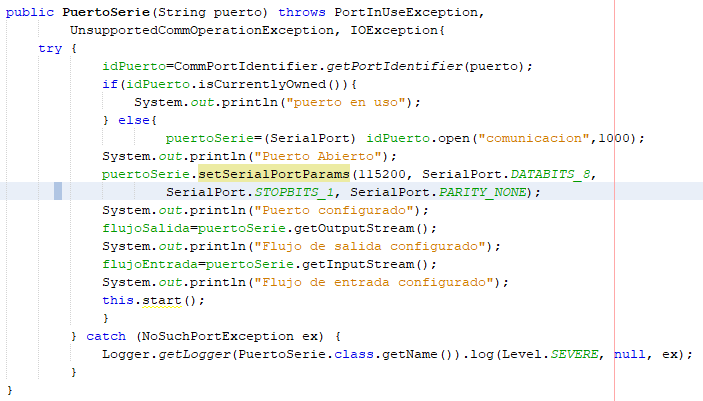
\includegraphics[scale=0.8]{Documento/Figuras/2.PNG}
\begin{scriptsize}
\\ 
\end{scriptsize}
\end{center}
Para la transmisión de información, declararemos un método con un argumento para transmitir el mensaje deseado, nos ayudaremos de un método .write() que posee la clase SerialPort.
\begin{center}
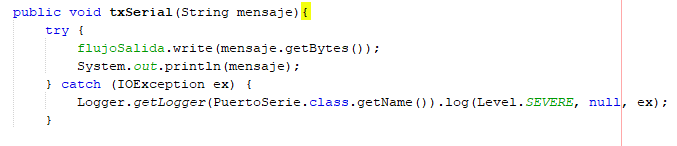
\includegraphics[scale=0.8]{Documento/Figuras/3.PNG}
\begin{scriptsize}
\\ 
\end{scriptsize}
\end{center}
Ahora para recibir datos usaremos un método run() de la clase derivada de Thread que nos permitirá crear un subproceso en el programa y con esto poner al puerto en constante “escucha”, por lo que necesitaremos crear un hilo hacia el constructor que contiene la información del puerto usado.
\begin{center}
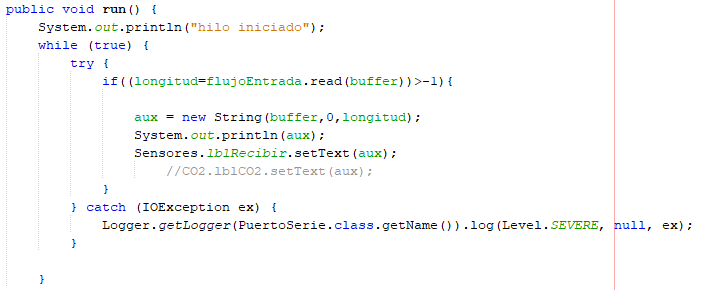
\includegraphics[scale=0.8]{Documento/Figuras/4.PNG}
\begin{scriptsize}
\\ 
\end{scriptsize}
\end{center}
Como usaremos varios sensores y actuares es necesario comunicarse con estos a través del puerto y luego cerrar dicha comunicación, ya que si esta quedara abierta, seria imposible comunicarse con varios sensores o actuadores a la vez, por lo que es necesario crear un método para cerrar los puertos usados.
\begin{center}
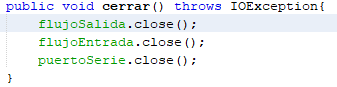
\includegraphics[scale=0.8]{Documento/Figuras/5.PNG}
\begin{scriptsize}
\\ 
\end{scriptsize}
\end{center}
Ahora necesitamos crear un Jframe para el control de esta clase, para este proyecto es necesario dos GUIs una que controlara los sensores y otra para controlar los actuadores.
Básicamente necesitamos colocar un ComboBox con el nombre de los puertos y un botón para activar la comunicación.
En el botón agregaremos un evento para que realice una acción al momento de ser presionado, esto nos permitirá escribir el código para activar la comunicación, para lo cual primero debemos crear un objeto de la clase que contiene los parámetros del Puerto serie y luego llamar los métodos necesarios para iniciar la comunicación, llevando la información obtenida del ComboBox y el mensaje deseado al momento de presionar el botón.
\begin{center}
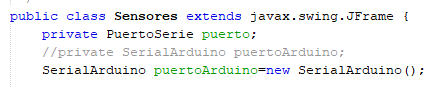
\includegraphics[scale=0.8]{Documento/Figuras/6.PNG}
\begin{scriptsize}
\\ 
\end{scriptsize}
\end{center}
\begin{center}
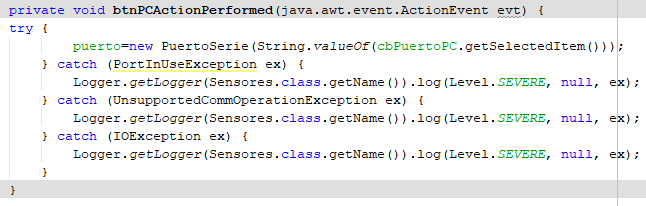
\includegraphics[scale=0.8]{Documento/Figuras/7.PNG}
\begin{scriptsize}
\\ 
\end{scriptsize}
\end{center}
\subsection{Comunicación con los actuadores}
Como es una comunicación cruzada, es necesario que en el software que controla los sensores tenga la capacidad de recibir los datos para controlar los actuadores, para ello se uso una clase muy similar a la de la Comunicación con el puerto serie, con la diferencia que se puso al puerto correspondiente de los actuadores en un subproceso de constante escritura de los datos recibidos por el otro computador.
\begin{center}
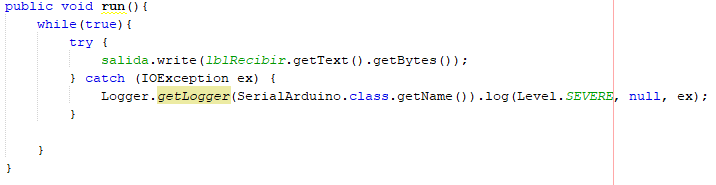
\includegraphics[scale=0.8]{Documento/Figuras/8.PNG}
\begin{scriptsize}
\\ 
\end{scriptsize}
\end{center}
\subsection{Comunicación con los sensores}
Para realizar la comunicación con los sensores debemos definir un nuevo se debe abrir y configurar un nuevo puerto en el que estará conectado nuestro arduino.
\begin{center}
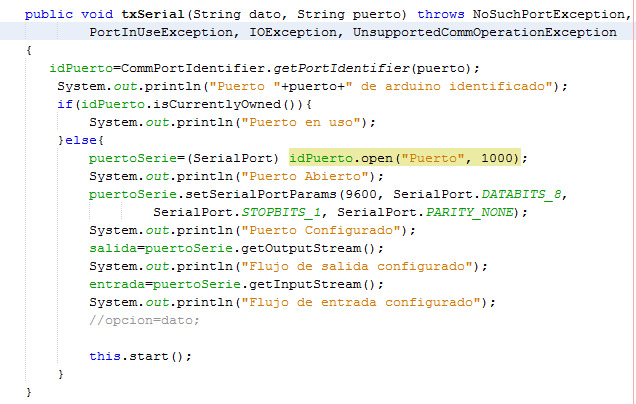
\includegraphics[scale=0.6]{Documento/Figuras/15.jpeg}
\begin{scriptsize}
\\ 
\end{scriptsize}
\end{center}

A continuación en el bucle infinito se procede a enviar un caracter al arduino de tal manera que en nuestro código arduino reconoce dicho caracter y retorna el valor que esta midiendo el sensor seleccionado.
\begin{center}
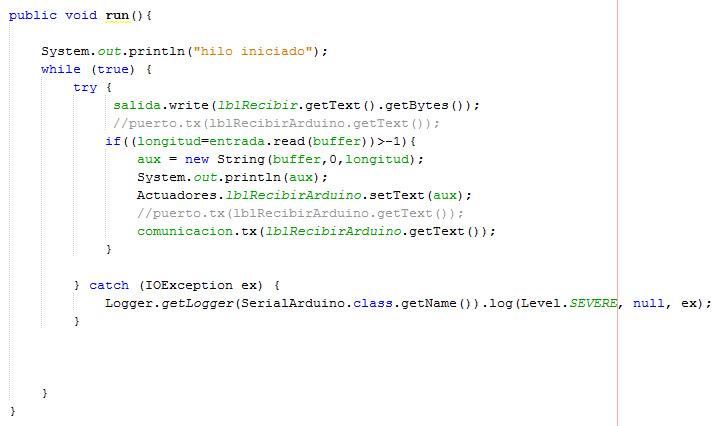
\includegraphics[scale=0.6]{Documento/Figuras/16.jpeg}
\begin{scriptsize}
\\ 
\end{scriptsize}
\end{center}

\subsection{Programación en Arduino}
\subsubsection{Actuadores}
Para los actuadores se uso una tarjeta ESP8266 la cual se puede programar en el IDE de Arduino, necesitamos manejar los pines digitales que posee la tarjeta, enviando un 0 o 1 logico para asi activar los controladores, estos controladores son: foco, niquelina, ventilador y un LCD. 
El foco necesita un circuito de control y uno de potencia, además de que la niquelina como el ventilador necesitan mas voltaje que el que entrega la tarjeta, por lo que usaremos transistores para amplificar la señal lógica que recibimos y de relés para controlar la parte de potencia, siguiendo el siguiente diagrama.
\begin{center}
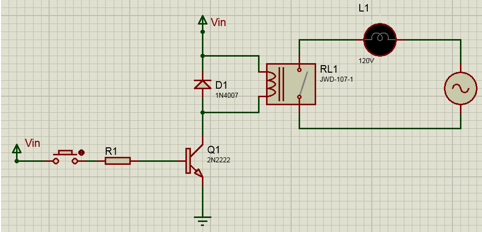
\includegraphics[scale=0.8]{Documento/Figuras/9.PNG}
\begin{scriptsize}
\\ 
\end{scriptsize}
\end{center}
Como se menciono antes, necesitaremos controlar un LCD para lo cual nos ayudamos de un modulo I2C por lo necesitaremos importar una librería al IDE de Arduino.
Luego procedemos a declarar los pines de la tarjeta en variables relacionadas con los actuadores a los que estarán conectados. 
En el void setup() empezaremos a declarar el modo en el que trabajaran los pines definidos anteriormente, en este caso todos serán OUTPUT (salida) y también se procedera a inicializar el lcd.
En el void loop() usaremos la condicion if-else, ya que en la comunicación en serie creada anteriormente, se transmitirán “caracteres” al momento de presionar los botones para activar o desactivar los dispositivos, por lo que necesitaremos comparar dichos caracteres recibidos con variables auxiliares. La lógica es que si estos caracteres recibidos son iguales a los comparados entrara en el laso if y ejecutara el comando para enviar un HIGH al pin seleccionado, y se seguirá esta lógica para todos los actuadores, pero para el lcd necesitaremos enviar el mensaje deseado, por lo que usaremos el comando lcd.print
\begin{center}
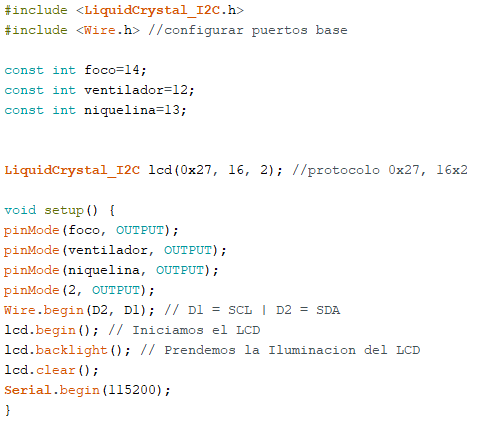
\includegraphics[scale=0.8]{Documento/Figuras/10.PNG}
\begin{scriptsize}
\\ 
\end{scriptsize}
\end{center}
\begin{center}
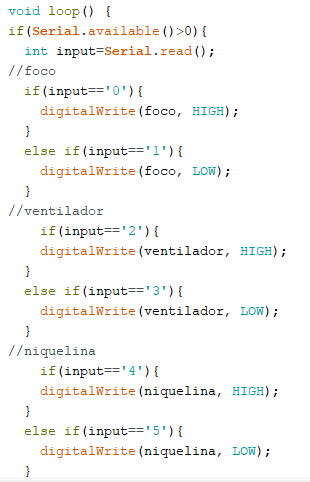
\includegraphics[scale=0.8]{Documento/Figuras/11.PNG}
\begin{scriptsize}
\\ 
\end{scriptsize}
\end{center}

\subsubsection{Sensores}
Para los sensores se usó una tarjeta Arduino UNO,  y de igual manera necesitaremos controlar los pines digitales y también los analógicos para recibir los datos obtenidos por los sensores.
Se procede a declarar los pines de la tarjeta en variables relacionadas con los sensores a los que estarán conectados. 
En el void setup() empezaremos a declarar el modo en que trabajaran los pines definidos anteriormente, en este caso necesitaremos que sean INPUT (entrada) y un OUTPUT (salida)
En el void loop() seguiremos la misma lógica que en los actuadores, vamos a comparar los caracteres recibidos por la comunicación serial y las compararemos mediante variables auxiliares para así entrar al laso if-else que contendrán los métodos necesarios para el funcionamiento de los sensores.
\begin{center}
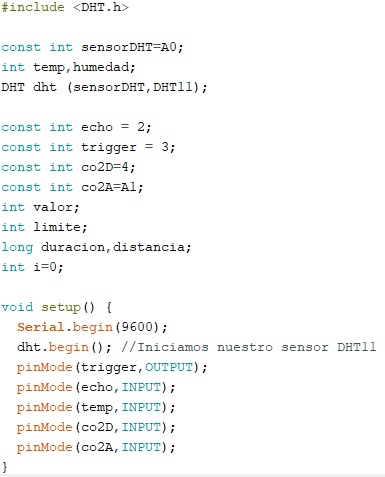
\includegraphics[scale=0.8]{Documento/Figuras/12.PNG}
\begin{scriptsize}
\\ 
\end{scriptsize}
\end{center}
\begin{center}
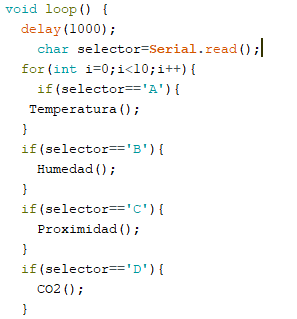
\includegraphics[scale=0.8]{Documento/Figuras/13.PNG}
\begin{scriptsize}
\\ 
\end{scriptsize}
\end{center}
\begin{center}
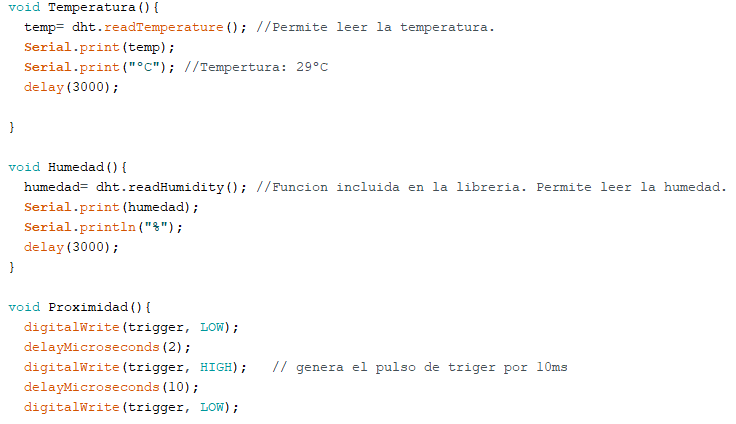
\includegraphics[scale=0.8]{Documento/Figuras/14.PNG}
\begin{scriptsize}
\\ 
\end{scriptsize}
\end{center}


 \section{CONCLUSIONES}
 \begin{itemize}
     \item La comunicación de puerto serial ha tenido una breve evolución en las últimas décadas, a través del estado del arte se comprobó su aplicación y funcionamiento con la transmisión de datos, en la creación del sistema de comunicación serial presentado en este informe, se procedió a la conexión entre dos computadoras con el Arduino y el uso del ESP8266, enviando datos para realizar la comunicación serial tanto para los sensores y los actuadores, por medio de una consola de java y Arduino.
     \item El Arduino se puede utilizar para diferentes ámbitos como desarrollar elementos autónomos, conectándose a dispositivos e interactuar tanto con el hardware como con el software; es una plataforma electrónica que en este trabajo nos permitió la interacción con una interfaz gráfica desarrollada con lenguaje de programación Java, con la finalidad de poder tener una interacción más fácil del Arduino con el computador.
     \item Se logro cumplir con cada uno de los objetivos, y entender el desarrollo de todos los programas, implementados en dos computadoras, con el debido funcionamiento de los Sensores y Actuadores.
 \end{itemize}

 \section{RECOMENDACIONES}
\begin{itemize}
    \item Se debe considerar que los pines en los que se conecta cada uno de los sensores y actuadores, que están configurados para funcionar en un orden específico, para obtener los datos requeríos en el Producto de unidad.
    \item Se debe tener en consideración que los paquetes utilizados en Java, no son propios de ahí, pero se debe descargar las librerias, y el funcionamiento de código nos permita trabajar de manera eficaz en los programas implementados..
    \item Conectar correctamente nuestros elementos, tanto a la tarjeta de Desarrollo del ESP8266 y la tarjeta de desarrollo Arduino UNO, debido a que, aunque realicemos correctamente la programación y la configuración con el servidor, los Actuadores y sensores se encuentran en los pines incorrectos o con la polarización indebida estos no podrán funcionar como esperamos.
\end{itemize}




%----------
%----------------------TABLAS-------------
%Insertar tabla
% Las tablas se pueden genederar a través de:
% www.tablegenerator.com
%---------------------------------------------------




%-------------------------------------------------------------------------------
% REFERENCIAS
%-------------------------------------------------------------------------------
\newpage

\begin{thebibliography}{99}

\bibitem{1}A., P. (17 de 10 de 2012). twenergy. Recuperado el 04 de 28 de 2018, de https://twenergy.com/a/como-se-genera-la-electricidad-666

\bibitem{2}Albatish, I., Mosa, M., & Abu , S. (01 de 2018). ResearchGate. Obtenido de 323322871_ARDUINO_Tutor_An_Intelligent_Tutoring_System

\bibitem{3}BBVA Open4U. (15 de 08 de 2015). BBVA. Obtenido de https://bbvaopen4u.com/es/actualidad/el-internet-de-las-cosas-de-codigo-abierto-plataformas-y-aplicaciones-para

\bibitem{4}Carlos, C. (12 de 06 de 2015). Galia,FC. Obtenido de http://galia.fc.uaslp.mx/

\bibitem{5}Cisco systems. (03 de 2016). ResearchGate. Obtenido de https://www.researchgate.net/publication/

\bibitem{6}Crespo, E. (25 de 09 de 2016). Aprendiendo Arduino. Obtenido de https://aprendiendoarduino.wordpress.com/2016/09/25/que-es-arduino/

\bibitem{7} Facultad Tecnológica. (02 de 10 de 2014). Universidad Distrital Francisco José de Caldas. Recuperado el 28 de 04 de 2018, de http://gemini.udistrital.edu.co/comunidad/grupos/gispud/Circuitos-II/Capitulo-3/3.2.1.html

\bibitem{8}García, J. A. (s.f.). AF. Obtenido de AF: http://www.asifunciona.com/fisica/af_diodos/af_diodos_6.htm

\bibitem{9}N.O.Sadiku, C. K. (2013). En Fundamentos de Circuitos Eléctricos (pág. 866). México: Mc Graw Hill Education
\end{thebibliography}

\section{ANEXOS}
 \begin{center}
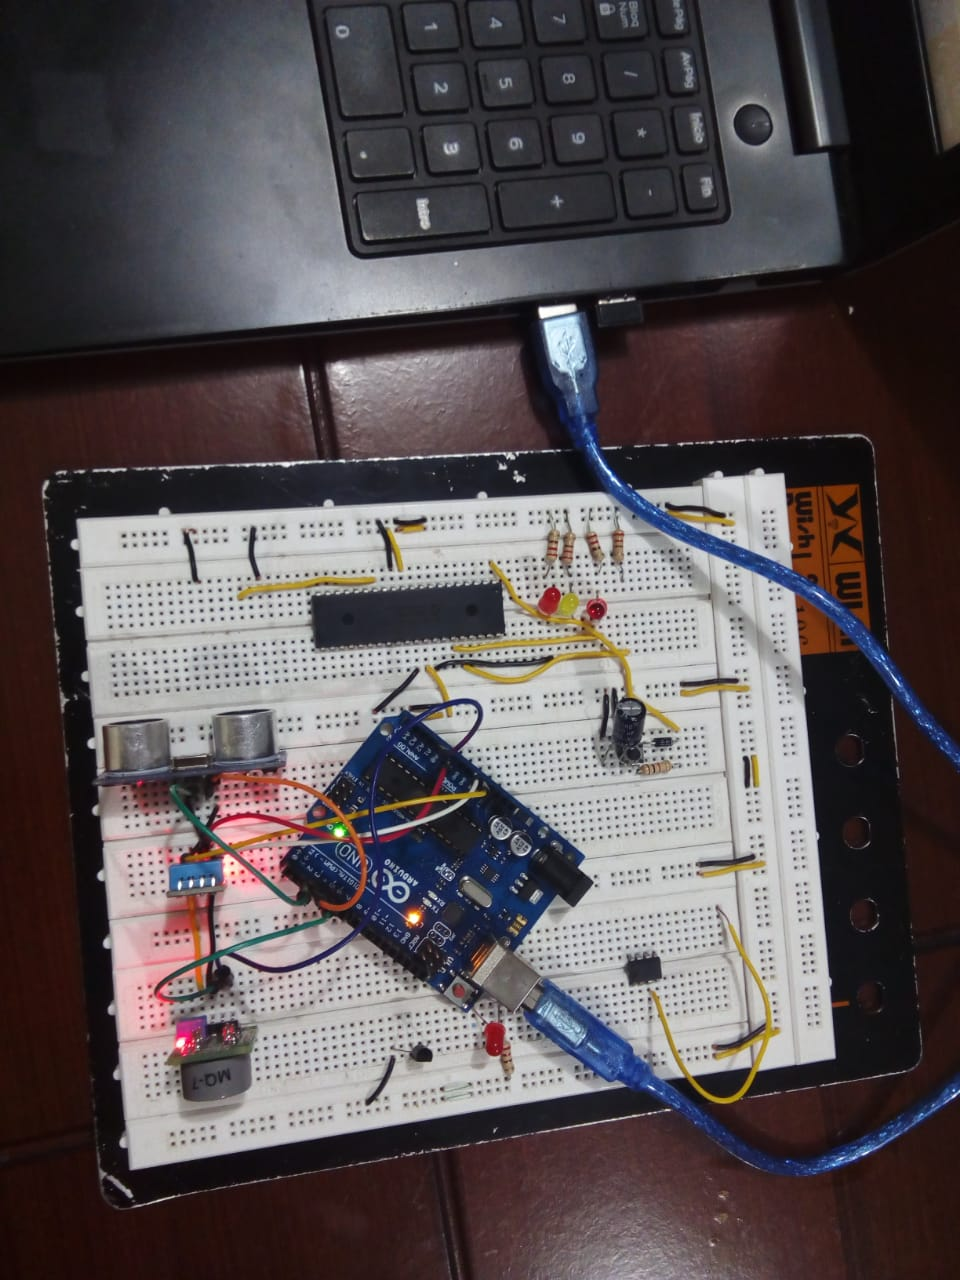
\includegraphics[scale=0.25]{Documento/Figuras/Sensores.jpeg}
\begin{scriptsize}\\ 
Fig 7. Sensores
\end{scriptsize}
\end{center}

 \begin{center}
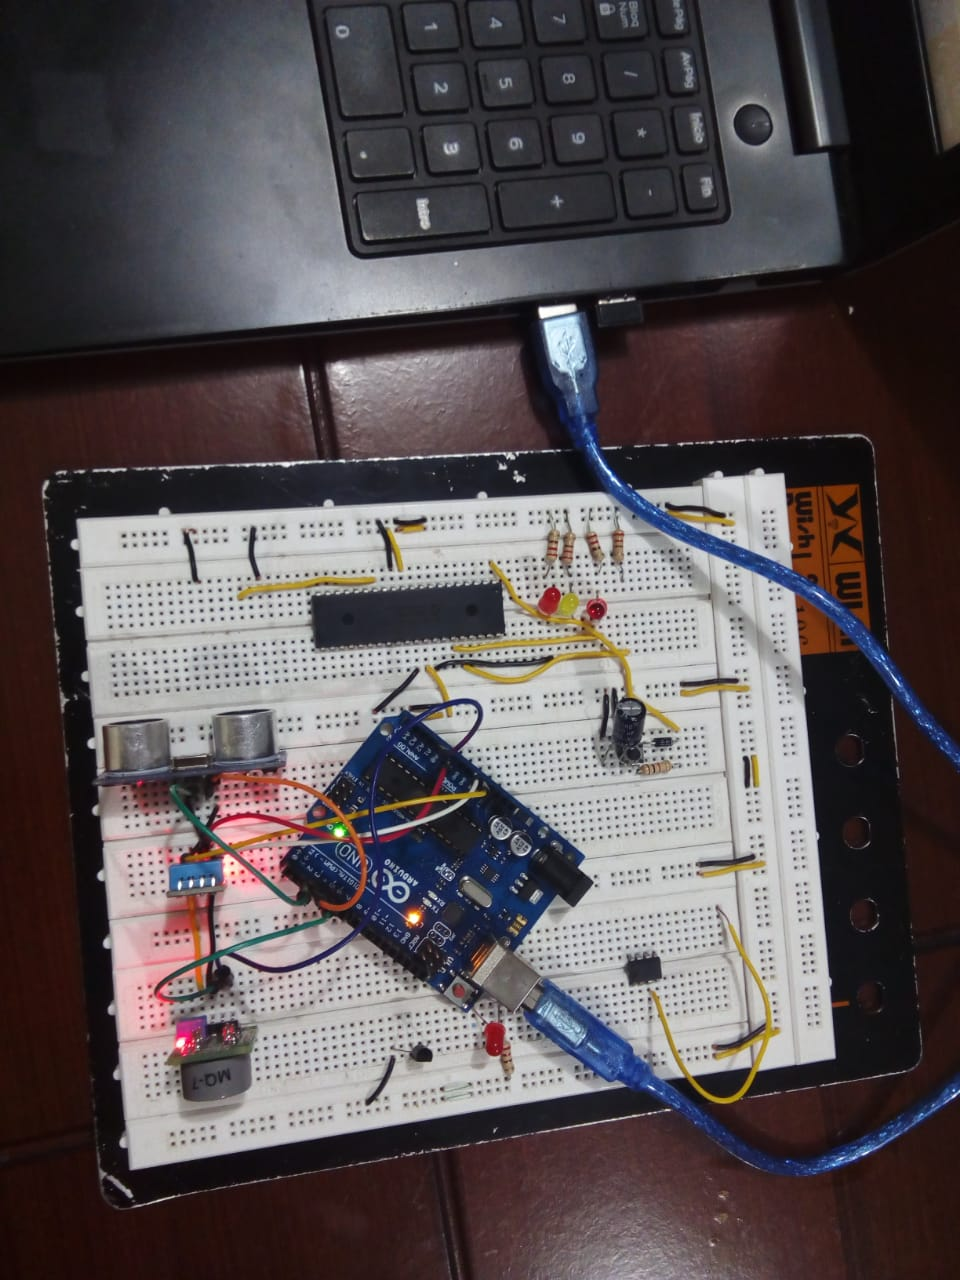
\includegraphics[scale=0.25]{Documento/Figuras/Sensores.jpeg}
\begin{scriptsize}\\ 
Fig 7. Actuadores
\end{scriptsize}
\end{center}

\end{document}



